\chapter{Lezione 10} \label{chap:lezione_10}
\begin{flushright}
\textit{Data: 24/10/2025} 
\end{flushright}

Nelle lezioni precedenti ci siamo concentrati sulle proprietà statiche dei sistemi. Introduciamo ora la \textbf{dinamica}, un passo fondamentale per due motivi principali:
\begin{enumerate}
    \item \textbf{Campionamento algoritmico:} Per studiare numericamente un sistema (es. Monte Carlo), è necessario definire una regola di evoluzione temporale che permetta di visitare lo spazio delle configurazioni e raggiungere l'equilibrio termodinamico (termalizzazione).
    \item \textbf{Fisica del non-equilibrio:} Vogliamo comprendere come un sistema evolve fisicamente quando viene preparato in uno stato iniziale lontano dall'equilibrio (ad esempio, un \textit{quench} da temperatura infinita a $T < T_c$).
\end{enumerate}

La grandezza fisica centrale in questo studio è la \textbf{lunghezza di correlazione dipendente dal tempo}, $\xi(t)$.

\section{ Lunghezza di Correlazione}
La dinamica nei modelli ordinati evolve e fa crescere la lunghezza di correlazione $\xi(t)$ in funzione del tempo. Nei modelli ordinati, se la lunghezza di correlazione iniziale è piccola, essa tenderà a crescere indefinitamente finché non subentra un fattore limitante (come la termalizzazione o la taglia del sistema).
In generale, il raggio di correlazione cresce nel tempo come una legge di potenza:
\begin{equation}
\xi(t) \sim t^{1/z}
\end{equation}
dove $z$ è noto come \textbf{esponente critico dinamico}. Il valore più comune e "classico" che si osserva in teorie gaussiane o nel modello di Ising 1D è $z=2$. Per sistemi disordinati come gli \textit{Spin Glasses}, la dinamica è molto più lenta ("sluggish") a causa della frustrazione. Al punto critico, l'esponente dinamico assume valori molto elevati, $z \approx 6 \div 7$, indicando un rilassamento estremamente lento.

\begin{tcolorbox}[colback=colorB!10, colframe=colorB!75!colorA, coltitle=white, title=\textbf{Dinamica all'Equilibrio vs Fuori dall'Equilibrio}]
\begin{itemize}
    \item \textbf{Dinamica all'equilibrio:} Si parte da condizioni iniziali distribuite secondo la misura di Gibbs-Boltzmann. Il sistema si evolve, ma macroscopicamente e statisticamente rimane all'equilibrio. La funzione di correlazione a due tempi dipende solo dalla differenza temporale $c(t, t') = \tilde{c}(t-t')$ in virtù dell'invarianza per traslazioni temporali. Il decadimento è descritto da un unico tempo caratteristico $\tau_{eq} \sim \xi_{eq}^z$.
    \item \textbf{Dinamica fuori dall'equilibrio:} Si parte da una configurazione iniziale generica (spesso random e uniforme). La lunghezza di correlazione dinamica $\xi(t)$ cresce progressivamente fino a raggiungere l'equilibrio $\xi_{eq}$ se la temperatura $T>0$, o prosegue se $T=0$.
\end{itemize}
\end{tcolorbox}

\subsection{Effetti di Taglia Finita}
L'evoluzione temporale della lunghezza di correlazione è limitata da due scale spaziali fondamentali: la taglia del sistema $L$ e la lunghezza di correlazione di equilibrio $\xi_{eq}(T)$. Possiamo distinguere tre regimi, illustrati schematicamente nel grafico log-log (Fig. \ref{fig:scaling_xi}).

\begin{figure}[h!]
\centering
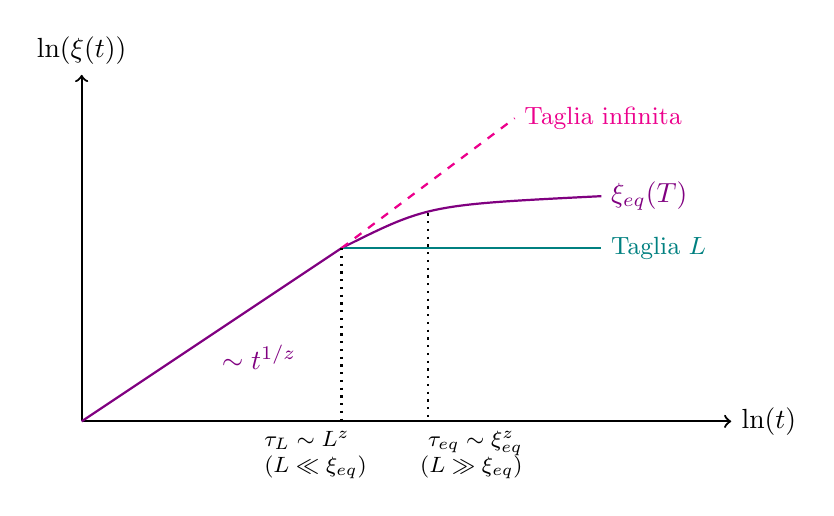
\begin{tikzpicture}[scale=1.1]
    % Assi (Estesi leggermente per far stare le etichette)
    \draw[->, thick] (0,0) -- (7.5,0) node[right] {$\ln(t)$};
    \draw[->, thick] (0,0) -- (0,4) node[above] {$\ln(\xi(t))$};
    
    % Crescita libera
    \draw[thick, violet] (0,0) -- (3, 2) node[midway, below right] {$\sim t^{1/z}$};
    
    % Saturazione Equilibrio (Curva Viola)
    \draw[thick, violet] (3,2) .. controls (4, 2.5) .. (6, 2.6);
    \node[right, violet] at (6, 2.6) {$\xi_{eq}(T)$};
    
    % Taglia Finita (Linea Teal)
    \draw[thick, teal] (3,2) -- (6, 2);
    \node[right, teal, font=\small] at (6, 2) {Taglia $L$};
    
    % Taglia Infinita (Linea Tratteggiata Magenta)
    \draw[dashed, magenta, thick] (3,2) -- (5, 3.5);
    \node[right, magenta, font=\small] at (5, 3.5) {Taglia infinita};

    % --- AGGIUNTA SCALE TEMPORALI ---
    
    % 1. Tempo di saturazione per Taglia Finita (tau_L)
    % Corrisponde al gomito a (3,2)
    \draw[dotted, black, thick] (3,2) -- (3,0);
    \node[below, align=left, font=\footnotesize] at (2.7,0) {$\tau_L \sim L^z$\\($L \ll \xi_{eq}$)};

    % 2. Tempo di saturazione per Equilibrio (tau_eq)
    % Corrisponde a quando la curva viola raggiunge il plateau (circa x=5.5 visivamente)
    \draw[dotted, black, thick] (4, 2.4) -- (4,0);
    \node[below, align=right, font=\footnotesize] at (4.5,0) {$\tau_{eq} \sim \xi_{eq}^z$\\($L \gg \xi_{eq}$)};

\end{tikzpicture}

\caption{Diagramma schematico (Log-Log) dell'evoluzione della lunghezza di correlazione $\xi(t)$. La crescita iniziale segue la legge di potenza $t^{1/z}$ (con $z=2$ per Ising 1D) fino a quando non intercetta la scala temporale dettata dalla lunghezza di equilibrio $\xi_{eq}$ o dalla taglia del sistema $L$.}
\label{fig:scaling_xi}
\end{figure}

Il tempo necessario a \textbf{decorrelare} o \textbf{termalizzare} segue una legge di scaling che dipende dal rapporto tra $L$ e $\xi_{eq}$:
\begin{equation}
    \tau(L, T) = L^z f\left( \frac{\xi_{eq}(T)}{L} \right) \approx
    \begin{cases}
        L^z & \text{se } L \ll \xi_{eq} \quad (\text{Regime di Taglia Finita}) \\
        \xi_{eq}^z & \text{se } L \gg \xi_{eq} \quad (\text{Regime Termodinamico})
    \end{cases}
\end{equation}

$\tau$ subisce un "cutoff" se il sistema ha dimensione lineare finita $L$. 

\noindent Quando $L \gg \xi_{eq}$, dopo un tempo $\tau_{eq}$, il sistema entra nel regime di equilibrio. Qui, le osservabili non evolvono più in media, ma fluttuano. La dinamica è descritta dalla funzione di autocorrelazione temporale:
\begin{equation}
    C(t, t') \sim e^{-(t-t')/\tau_{eq}}
\end{equation}



\section{Dinamica di Glauber per Ising 1D}
Analizziamo esplicitamente la dinamica di Glauber nel modello di Ising unidimensionale in assenza di campo magnetico esterno ($h=0$). 

\noindent L'Hamiltoniana è ($J=1$):
\begin{equation}
    H = - \sum_i S_i S_{i+1}
\end{equation}

\noindent Definiamo il \textbf{campo locale} $h_i$ agente sullo spin $i$:
\begin{equation}
    h_i = S_{i-1} + S_{i+1}
\end{equation}

\noindent La probabilità di transizione per lo spin $i$ di assumere valore $S$ al tempo $t+1$ è data da:
\begin{equation}
    \mathbb{P}(S_i(t+1) = S) = \frac{1 + S \tanh(\beta h_i)}{2}
\end{equation}


\noindent L'evoluzione della probabilità $P(\vec{s}, t)$ della configurazione totale al tempo $t$ è data dalla \textbf{Master Equation}:
\begin{equation}
\frac{d P(\vec{s}, t)}{dt} = \sum_{i} P(\vec{s}^{(i)}, t) \frac{1 + s_i \tanh(\beta h_i)}{2} - P(\vec{s}, t) \sum_{i} \frac{1 - s_i \tanh(\beta h_i)}{2}
\end{equation}
dove $\vec{s}^{(i)} = (s_1, \dots, -s_i, \dots, s_N)$ indica la configurazione che differisce da $\vec{s}$ esclusivamente per il ribaltamento dell'i-esimo spin. 

\noindent Il primo termine rappresenta il flusso di probabilità in entrata nello stato $\vec{s}$ (partendo dagli stati adiacenti), mentre il secondo termine rappresenta il flusso in uscita verso altri stati.

La Master Equation mantiene conservata la probabilità totale.

\subsection{Dinamica della Correlazione Spaziale}
Poiché la risoluzione esatta della Master Equation per l'intera distribuzione di probabilità $P(\vec{s}, t)$ in un sistema macroscopico risulta impraticabile, è conveniente proiettare l'evoluzione dinamica su un'osservabile scalare. Una scelta fisicamente rilevante è la funzione di correlazione spaziale a due punti:
\begin{equation}
    C_{ij}(t) = \sum_{\vec{s}} P(\vec{s}, t) S_i S_j
\end{equation}
Assumendo l'invarianza per traslazioni spaziali, questa quantità dipende unicamente dalla distanza relativa $r = |i - j|$. Fissando un sito di riferimento nell'origine, definiamo l'osservabile di interesse come:
\begin{equation}
    G(r, t) = \langle C_{0r}(t) \rangle = \sum_{\vec{s}} P(\vec{s}, t) S_0 S_r
\end{equation}
La media è sulle traiettorie e sulla condizione iniziale. Si parte da una condizione iniziale disordinata $G(r, 0) = \delta_{r, 0}$.

Per derivare l'equazione di evoluzione di $G(r, t)$, moltiplichiamo la Master Equation per $S_0 S_r$ e sommiamo su tutte le configurazioni:
\begin{equation}
    \frac{d}{dt} G(r, t) = \sum_{\vec{s}} S_0 S_r \left[ \sum_{i} P(\vec{s}^{(i)}, t) \frac{1 + S_i \tanh(\beta h_i)}{2} - P(\vec{s}, t) \sum_{i} \frac{1 - S_i \tanh(\beta h_i)}{2} \right]
\end{equation}
dove $\vec{s}^{(i)}$ indica la configurazione in cui lo spin $i$-esimo è stato invertito.

La sommatoria su tutti i siti $i$ può essere semplificata analizzando le proprietà dell'osservabile $S_0 S_r$. Considerando il primo termine in parentesi (che rappresenta la probabilità di transizione in "entrata") ed effettuando il cambio di variabili $\vec{\tau} = \vec{s}^{(i)}$, si valuta formalmente l'effetto del flip del singolo spin nel sito $i$-esimo. 

Si distinguono due casi per l'indice di sommatoria:
\begin{itemize}
    \item \textbf{Se $\mathbf{i \neq 0}$ e $\mathbf{i \neq r}$:} il flip avviene in un sito non coinvolto nell'osservabile. Di conseguenza, gli spin $S_0$ e $S_r$ non vengono alterati dalla trasformazione e il loro prodotto rimane invariato. In queste condizioni, il termine di entrata e il termine di uscita assumono lo stesso valore assoluto ma segno opposto, elidendosi esattamente.
    \item \textbf{Se $\mathbf{i = 0}$ o $\mathbf{i = r}$:} il flip coinvolge direttamente uno degli spin dell'osservabile, invertendone il segno. Questo cambio di segno fa sì che i termini di entrata e uscita non si cancellino.
\end{itemize}

La sommatoria spaziale su tutti gli $N$ siti del reticolo si riduce quindi ai soli due contributi non nulli nei siti $i = 0$ e $i = r$. Poiché il modello in assenza di campo esterno è invariante per traslazioni spaziali, l'effetto statistico del flip nel sito $0$ è equivalente a quello nel sito $r$. Sfruttando questa simmetria, è sufficiente calcolare il termine per $i = r$ e moltiplicarlo per 2, ottenendo:
\begin{equation}
    \frac{d}{dt} G(r, t) = - \sum_{\vec{s}} S_0 S_r P(\vec{s}, t) \left( 1 - S_r \tanh(\beta h_r) \right)
\end{equation}

Nel modello di Ising unidimensionale, il campo locale $h_r = S_{r-1} + S_{r+1}$ assume solo i valori $0, \pm 2$. Questa peculiarità permette di linearizzare esattamente la tangente iperbolica sul reticolo:
\begin{equation}
    \tanh(\beta(S_{r-1} + S_{r+1})) = \frac{S_{r-1} + S_{r+1}}{2} \tanh(2\beta)
\end{equation}
Sostituendo tale espressione e ricordando che $S_r^2 = 1$, l'equazione diventa:
\begin{equation}
    \frac{d}{dt} G(r, t) = - \sum_{\vec{s}} P(\vec{s}, t) S_0 S_r + \frac{\tanh(2\beta)}{2} \left[ \sum_{\vec{s}} P(\vec{s}, t) S_0 S_{r-1} + \sum_{\vec{s}} P(\vec{s}, t) S_0 S_{r+1} \right]
\end{equation}
Riconoscendo le definizioni delle funzioni di correlazione e riordinando i termini in modo da evidenziare la struttura alle differenze finite spaziali, giungiamo all'equazione esatta sul reticolo:
\begin{equation}
    \frac{dG(r, t)}{dt} = -(1 - \tanh(2\beta)) G(r, t) + \frac{\tanh(2\beta)}{2} \left[ G(r-1, t) - 2G(r, t) + G(r+1, t) \right]
\end{equation}
Nel limite del continuo (per distanze $r$ sufficientemente grandi), il termine in parentesi quadra corrisponde alla derivata seconda spaziale $\frac{\partial^2 G(r,t)}{\partial r^2}$.

\subsubsection{Limiti Fisici e Scaling di Porod}
Possiamo estrarre informazioni cruciali studiando i limiti asintotici di questa equazione:
\begin{enumerate}
    \item \textbf{Regime stazionario all'equilibrio ($t \to \infty, T > 0$):}\\
     Il sistema stazionarizza e la derivata temporale si annulla ($\frac{\partial G}{\partial t} = 0$). Sostituendo nella versione continua, si ottiene:
    \begin{equation}
        (1 - \tanh(2\beta)) G_{eq}(r) = \frac{\tanh(2\beta)}{2} \frac{\partial^2 G_{eq}}{\partial r^2}
    \end{equation}
    Dall'analisi dimensionale di questa equazione differenziale ricaviamo la lunghezza di correlazione all'equilibrio $\xi_{eq}$:
    \begin{equation}
        \xi_{eq}^2 \propto \frac{\tanh(2\beta)}{1 - \tanh(2\beta)} \sim e^{4\beta} \quad \text{per } T \ll 1
    \end{equation}
    Questo risultato coincide perfettamente con la divergenza nota della lunghezza di correlazione per il modello di Ising unidimensionale, confermando l'esattezza dell'approccio.
    

    \item \textbf{Dinamica fuori dall'equilibrio ($T = 0$):}\\
    A temperatura nulla il sistema non raggiunge mai l'equilibrio perché $\xi_{eq} \to \infty$. Sostituendo $\tanh(2\beta) = 1$, il termine di decadimento lineare si annulla e ci ritroviamo con una pura \textbf{equazione della diffusione}:
    \begin{equation}
        \frac{d G(r, t)}{dt} = \frac{1}{2} \frac{\partial^2 G(r, t)}{\partial r^2}
    \end{equation}
    Dimensionalmente, affinché $r^2$ scali come $t$, dobbiamo avere un andamento per la lunghezza di correlazione $\xi(t) \sim t^{1/2}$. Questo identifica l'esponente critico dinamico $z = 2$. Inserendo una forma di scaling $\tilde{G}(r / t^{1/2})$ nell'equazione, la soluzione analitica esatta restituisce la \textbf{Legge di Porod}:
    \begin{equation}
        G(r, t) = 1 - \text{erf}\left( \frac{r}{2\sqrt{t}} \right) \quad \implies \quad \tilde{G}(z) = 1 - \text{erf}\left(\frac{z}{2}\right)
    \end{equation}
    
   Sviluppando in serie di Taylor la funzione di errore per argomenti piccoli, la funzione di correlazione esibisce una dipendenza strettamente lineare: $G(r, t) \approx 1 - \frac{r}{\sqrt{\pi t}}$

Di conseguenza, la derivata spaziale all'origine è finita e \textbf{non nulla}: $\left. \frac{\partial G}{\partial r} \right|_{r \to 0} \neq 0$

Graficamente, questo andamento si traduce in una \textbf{cuspide} in $r=0$.

\begin{itemize}
    \item \textbf{Modelli continui (es. teoria di Ginzburg-Landau):} Il parametro d'ordine varia nello spazio in modo differenziabile (``liscio''). La correlazione all'origine ha un andamento parabolico, il che impone una derivata rigorosamente nulla in $r=0$.
    
    \item \textbf{Modello di Ising (discreto):} Le variabili di spin sono rigorosamente discrete ($S_i = \pm 1$). Il passaggio tra domini di spin opposti è istantaneo (avviene in un singolo passo reticolare) e genera un'\textbf{interfaccia netta} (\textit{sharp interface}) priva di spessore, che costituisce fisicamente il \textbf{Domain Wall}.
\end{itemize}

Consideriamo due spin separati da una distanza piccolissima $r$. Essendo molto vicini, è altamente probabile che si trovino nello stesso dominio, fornendo un contributo alla correlazione pari a $1$. L'unico caso in cui i due spin risultano opposti (contributo pari a $-1$) si verifica se un \textit{Domain Wall} cade esattamente nello spazio che li separa.

Poiché nel modello di Ising le interfacce non hanno spessore, la probabilità di ``catturare'' un \textit{Domain Wall} in un piccolo intervallo è \textbf{direttamente proporzionale alla lunghezza dell'intervallo $r$}. È proprio questa probabilità a generare la dipendenza lineare $G(r) \approx 1 - c r \quad (c > 0)$, spiegando fisicamente la derivata non nulla e la presenza della cuspide all'origine.
\end{enumerate}

\section{Dinamica dei Difetti (Domain Walls)}
Un modo complementare, e fisicamente più illuminante, per studiare la \textbf{dinamica di coarsening} (\textbf{crescita dei domini ordinati} e coesistenza tra essi) è spostare il focus dalla configurazione degli spin all'evoluzione dei difetti di energia, chiamati \textbf{Domain Walls (DW)}.
Un DW si trova ovunque vi sia un'interazione violata (due spin adiacenti antiparalleli). Esiste una mappatura "quasi" biunivoca (c'è una degenerazione $Z_2$) tra le configurazioni degli spin e quelle dei DW.

Riprendendo le regole di Glauber in termini di probabilità termiche, identifichiamo tre processi stocastici per i DW, controllati da una scala di tempo universale associata a un rate di transizione globale $\Gamma$:

\begin{itemize}
    \item \textbf{Annichilazione:} Due DW adiacenti convergono e si distruggono. Probabilità dominata dalla forte preferenza termica di allineamento:\\
    \text{Rate } $\propto \Gamma [1 + \tanh(2\beta)]$
    \begin{center}
\begin{tikzpicture}[>=Stealth, thick, scale=0.8, every node/.style={transform shape}]
    \tikzstyle{spin} = [circle, draw=black, thick, minimum size=0.7cm, inner sep=0pt, font=\Large]
    \tikzstyle{dw} = [red, very thick, dashed]
    \tikzstyle{arrow} = [->, very thick, blue!80!black]

    % Stato iniziale
    \node[spin] (a1) at (0,0) {$+$};
    \node[spin] (a2) at (1,0) {$+$};
    \node[spin, fill=yellow!40] (a3) at (2,0) {$-$}; 
    \node[spin] (a4) at (3,0) {$+$};
    \node[spin] (a5) at (4,0) {$+$};
    
    \draw[dw] (1.5, 0.7) -- (1.5, -0.7) node[below] {\small DW};
    \draw[dw] (2.5, 0.7) -- (2.5, -0.7) node[below] {\small DW};

    % Freccia
    \draw[arrow] (4.8, 0) -- (6.2, 0) node[midway, above] {\small Flip};

    % Stato finale
    \begin{scope}[shift={(7, 0)}]
        \node[spin] (b1) at (0,0) {$+$};
        \node[spin] (b2) at (1,0) {$+$};
        \node[spin, fill=green!20] (b3) at (2,0) {$+$};
        \node[spin] (b4) at (3,0) {$+$};
        \node[spin] (b5) at (4,0) {$+$};
        \node[below, text=green!60!black, font=\small\bfseries] at (2, -0.7) {0 DW};
    \end{scope}
\end{tikzpicture}
\end{center}
    
    \item \textbf{Creazione:} Fluttuazione termica che spezza un dominio creando due DW. Estremamente improbabile a basse temperature:\\
    \text{Rate } $\propto \Gamma [1 - \tanh(2\beta)]$
    \begin{center}
\begin{tikzpicture}[>=Stealth, thick, scale=0.8, every node/.style={transform shape}]
    \tikzstyle{spin} = [circle, draw=black, thick, minimum size=0.7cm, inner sep=0pt, font=\Large]
    \tikzstyle{dw} = [red, very thick, dashed]
    \tikzstyle{arrow} = [->, very thick, blue!80!black]

    % Stato iniziale
    \node[spin] (c1) at (0,0) {$+$};
    \node[spin] (c2) at (1,0) {$+$};
    \node[spin, fill=yellow!40] (c3) at (2,0) {$+$}; 
    \node[spin] (c4) at (3,0) {$+$};
    \node[spin] (c5) at (4,0) {$+$};

    % Freccia
    \draw[arrow] (4.8, 0) -- (6.2, 0) node[midway, above] {\small Flip};

    % Stato finale
    \begin{scope}[shift={(7, 0)}]
        \node[spin] (d1) at (0,0) {$+$};
        \node[spin] (d2) at (1,0) {$+$};
        \node[spin, fill=red!20] (d3) at (2,0) {$-$};
        \node[spin] (d4) at (3,0) {$+$};
        \node[spin] (d5) at (4,0) {$+$};
        
        \draw[dw] (1.5, 0.7) -- (1.5, -0.7) node[below] {\small DW};
        \draw[dw] (2.5, 0.7) -- (2.5, -0.7) node[below] {\small DW};
    \end{scope}
\end{tikzpicture}
\end{center}
    \item \textbf{Spostamento:} Un DW compie un salto reticolare verso un sito adiacente neutro. È un puro \textbf{random walk} non ostacolato termicamente:\\
    \text{Rate } $\propto \Gamma$
    \begin{center}
\begin{tikzpicture}[>=Stealth, thick, scale=0.8, every node/.style={transform shape}]
    \tikzstyle{spin} = [circle, draw=black, thick, minimum size=0.7cm, inner sep=0pt, font=\Large]
    \tikzstyle{dw} = [red, very thick, dashed]
    \tikzstyle{arrow} = [->, very thick, blue!80!black]

    % Stato iniziale
    \node[spin] (e1) at (0,0) {$+$};
    \node[spin] (e2) at (1,0) {$+$};
    \node[spin, fill=yellow!40] (e3) at (2,0) {$-$}; 
    \node[spin] (e4) at (3,0) {$-$};
    \node[spin] (e5) at (4,0) {$-$};
    
    \draw[dw] (1.5, 0.7) -- (1.5, -0.7) node[below] {\small DW};

    % Freccia
    \draw[arrow] (4.8, 0) -- (6.2, 0) node[midway, above] {\small Flip};

    % Stato finale
    \begin{scope}[shift={(7, 0)}]
        \node[spin] (f1) at (0,0) {$+$};
        \node[spin] (f2) at (1,0) {$+$};
        \node[spin, fill=cyan!20] (f3) at (2,0) {$+$};
        \node[spin] (f4) at (3,0) {$-$};
        \node[spin] (f5) at (4,0) {$-$};
        
        \draw[dw] (2.5, 0.7) -- (2.5, -0.7) node[below] {\small DW};
        \draw[->, thick, cyan!80!black] (0.9, -1.0) -- (1.9, -1.0) node[midway, below] {\footnotesize Diffusione};
    \end{scope}
\end{tikzpicture}
\end{center}
\end{itemize}

A $T=0$, la probabilità di creazione si annulla. I difetti seguono quindi una cinematica governata unicamente dallo spostamento e dall'annichilazione. Due difetti separati da una distanza tipica $\xi(t)$ diffonderanno (random walk) e si annichileranno in un tempo proporzionale al quadrato della loro distanza, $t \sim \xi^2(t)$, riotteniamo quindi l'esponente dinamico $z=2$.


\subsection{Fallimento del Campo Medio e Pseudo-gap}
Definita $n(t)$ la densità spaziale dei DW,l'energia media del sistema risulta 
\begin{equation}
    \mathcal{E}(t) = -1 + 2n(t) 
\end{equation}
Se cerchiamo di descrivere l'evoluzione di $n(t)$ applicando l'approssimazione del \textbf{caos molecolare} (fattorizzando la probabilità di trovare due DW vicini come $n(t)^2$), otteniamo:
\begin{equation}
    \frac{1}{\Gamma}\frac{dn(t)}{dt} = [1 - \tanh(2\beta)] \big(1 - n(t)\big)^2 - [1 + \tanh(2\beta)] n(t)^2
\end{equation}
\subsubsection*{Analisi del limite stazionario ($t \to \infty$)}
Verifichiamo la validità dell'equazione all'equilibrio termodinamico annullando la derivata temporale ($\frac{dn(t)}{dt} = 0$):
\begin{equation}
    [1 - \tanh(2\beta)] (1 - n_{eq})^2 = [1 + \tanh(2\beta)] n_{eq}^2
\end{equation}
Dividendo entrambi i membri per $n_{eq}^2$ e per il termine $[1 - \tanh(2\beta)]$, si ottiene:
\begin{equation}
    \frac{(1 - n_{eq})^2}{n_{eq}^2} = \frac{1 + \tanh(2\beta)}{1 - \tanh(2\beta)}
\end{equation}
Estraendo la radice quadrata di ambo i membri (essendo $n_{eq} \ge 0$ e $1-n_{eq} \ge 0$):
\begin{equation}
    \frac{1 - n_{eq}}{n_{eq}} = \sqrt{\frac{1 + \tanh(2\beta)}{1 - \tanh(2\beta)}} \implies \frac{1}{n_{eq}} - 1 = \sqrt{\frac{1 + \tanh(2\beta)}{1 - \tanh(2\beta)}}
\end{equation}
Risolvendo rispetto a $n_{eq}$ si ricava la formula esatta per la densità di equilibrio:
\begin{equation}
    n_{eq} = \left( 1 + \sqrt{\frac{1 + \tanh(2\beta)}{1 - \tanh(2\beta)}} \right)^{-1}
\end{equation}

Esplicitando la tangente iperbolica e semplificando:
\begin{equation}
    m_{eq} = \left( 1 + \sqrt{e^{4\beta}} \right)^{-1} = \frac{1}{1 + e^{2\beta}} \sim e^{-2\beta} \sim \frac{1}{\xi_{eq}}
\end{equation}
Poiché a basse temperature la lunghezza di correlazione all'equilibrio si comporta come $\xi_{eq} \sim e^{2\beta}$, l'approssimazione di campo medio restituisce lo scaling termodinamico corretto per la densità dei difetti.

\subsubsection*{Analisi della dinamica fuori dall'equilibrio a $T=0$}
A temperatura zero ($T = 0$, ovvero $\beta \to \infty$), la creazione di difetti è impossibile e si ha $\tanh(2\beta) = 1$. 
Assorbendo le costanti, l'equazione cinetica assume la forma:
\begin{equation}
    \frac{dn(t)}{dt} = -2\Gamma n(t)^2
\end{equation}
Per tempi lunghi si ottiene il decadimento:
\begin{equation}
    n(t) \sim \frac{1}{t}
\end{equation}
Questo andamento temporale entra in palese contraddizione con lo scaling spaziale corretto, per il quale la densità dei difetti deve decrescere come l'inverso della lunghezza di correlazione dinamica:
\begin{equation}
    n(t) \propto \frac{1}{\xi(t)} \sim \frac{1}{t^{1/2}}
\end{equation}

\vspace{0.3cm}

\noindent L'errore fondamentale che genera questa discrepanza risiede nell'ipotesi del caos molecolare. Il processo di annichilazione elimina sistematicamente i difetti adiacenti, creando forti correlazioni spaziali a corto raggio. La dinamica dei DW non è descritta da cammini casuali indipendenti, ma si comporta come un \textbf{Random Walk in presenza di una Parete Assorbente} (che simula l'annichilazione istantanea all'incontro). 

Mentre in un cammino casuale libero la densità di probabilità all'origine $P(0)$ assume un valore finito, la presenza della condizione assorbente schiaccia linearmente a zero la probabilità a corte distanze. Si genera così uno \textbf{pseudo-gap}.
Questa riduzione locale di probabilità rende gli incontri tra i difetti meno frequenti. Di conseguenza, la probabilità che due DW si trovino vicini per annichilirsi non scala come $n(t)^2$, ma subisce una soppressione che la fa variare come $n(t)^3$.
L'equazione cinetica assume quindi una forma cubica, da cui segue:
\begin{equation}
     n(t) \sim \frac{1}{t^{1/2}}
\end{equation}
Questo risultato teorico ristabilisce la piena coerenza fisica con la legge di accrescimento diffusivo dei domini $\xi(t) \sim t^{1/2}$, confermando l'esponente dinamico $z=2$.

\vspace{0.5cm}

\begin{figure}[H]
\centering
\begin{tikzpicture}[>=Stealth, scale=1.3, thick]
    % Assi
    \draw[->, very thick] (0,0) -- (6,0) node[right] {$x$};
    \draw[->, very thick] (0,0) -- (0,4) node[above] {$P$};

    % RW Libero
    \draw[violet, thick] (0, 3.5) node[above right] {RW Libero} .. controls (2, 3.5) and (3, 1) .. (5, 0.2) ;

    % RW Assorbente
    \draw[red, thick] (0, 0) -- (0.8, 1.5) .. controls (1.5, 2.5) and (2.5, 2.5) .. (3.5, 1) .. controls (4, 0.5) and (4.5, 0.2) .. (5, 0.1) node[above right, text=red] {RW Assorbente};

    \node[anchor=north west] at (0.2, 3) {\color{violet} $P(0) \neq 0$};
    \node[anchor=north west] at (1.2, 1.2) {\color{red} \textit{Pseudo-gap}};
\end{tikzpicture}
\caption{Distribuzione spaziale per modelli di Random Walk. Nel RW libero la probabilità di prossimità è massima all'origine. Nel caso dei Domain Walls, l'annichilazione agisce come parete assorbente, generando uno pseudo-gap lineare che sopprime fortemente la probabilità di incontro a distanze brevi.}
\end{figure}

\newpage
\section{Modello di Ginzburg-Landau Dipendente dal Tempo (TDGL)}

Nei modelli di Ising unidimensionali l'analisi reticolare esatta è fattibile, ma estenderla a $D > 1$ (sistemi bidimensionali o tridimensionali) diviene analiticamente impossibile fuori dall'equilibrio.
Per catturare la fisica universale di questi sistemi, si passa a un approccio di teoria dei campi, definendo un'equazione stocastica differenziale per il parametro d'ordine continuo (o campo) $\Phi(\vec{x}, t)$, nota come \textbf{Equazione di Ginzburg-Landau dipendente dal tempo (TDGL)}:
\begin{equation}
    \frac{1}{\Gamma} \frac{\partial \Phi}{\partial t} = -\frac{\delta F[\Phi]}{\delta \Phi(\vec{x}, t)} + \eta(\vec{x}, t)
\end{equation}
Il termine $-\frac{\delta F}{\delta \Phi}$ spinge il campo a minimizzare l'energia libera per rilassare verso l'equilibrio termodinamico, mentre $\eta(\vec{x}, t)$ è un rumore termico bianco (delta-correlato sia in spazio che in tempo) che descrive le fluttuazioni stocastiche introdotte dalla temperatura.

Prendiamo in esame un funzionale di Landau per una \textbf{teoria gaussiana}, ovvero il propagatore libero senza termini quartici di rottura di simmetria:
\begin{equation}
    F[\Phi] = \int d^D \vec{x} \left( \frac{1}{2} |\nabla \Phi|^2 + \frac{m^2}{2} \Phi^2 \right) - h\Phi
\end{equation}
L'equazione differenziale risultante per il punto di sella è rigorosamente lineare nel campo. Possiamo diagonalizzarla introducendo la trasformata di Fourier nello spazio reciproco dei momenti $\vec{k}$ e delle frequenze $\omega$ ($\Phi(\vec{x}, t) \to \hat{\Phi}(\vec{k}, \omega)$):
\begin{equation}
    \left( - \frac{i\omega}{\Gamma} + k^2 + m^2 \right) \hat{\Phi}(\vec{k}, \omega) = \hat{h} + \hat{\eta}
\end{equation}

Da questa relazione strutturale estraiamo la \textbf{suscettività generalizzata} mediando rispetto al campo ausiliario $\hat{h}$:
\begin{equation}
    \frac{\partial \langle \hat{\Phi} \rangle}{\partial \hat{h}} = \frac{\Gamma}{-i\omega + \Gamma(k^2 + m^2)} 
\end{equation}
Per evidenziare le proprietà universali di invarianza di scala, riorganizziamo i termini fattorizzando il vettore d'onda $k^2$ al denominatore e assorbendo le costanti. La suscettività (o equivalentemente il suo inverso $\chi^{-1}$) può essere riformulata come una funzione di puro scaling:
\begin{equation}
    \chi^{-1} \propto k^2 f\left( \frac{m}{k}, \frac{\omega}{k^2} \right)
\end{equation}


Affinché gli argomenti della funzione $f$ siano quantitativamente adimensionali, la frequenza $\omega$ deve necessariamante scalare con il quadrato del vettore d'onda $k$. Questo dimostra in modo universale, indipendente dalla dimensionalità del sistema, che per modelli ordinati analizzabili in campo medio (teoria gaussiana) l'esponente critico dinamico è rigidamente \textbf{$z = 2$}.

In sistemi reali al punto critico, l'integrazione delle fluttuazioni (gruppo di rinormalizzazione) induce lievi correzioni all'esponente (es. $z \approx 2.15$ in 3D). Tali dinamiche si distinguono in modo diametrale dalla classe di universalità dei sistemi disordinati (\textit{Spin Glasses}), nei quali la frustrazione topologica del panorama energetico eleva l'esponente dinamico a scale di gran lunga superiori ($z \approx 6 \div 7$), rallentando drasticamente il rilassamento del sistema.




